\documentclass[1p]{elsarticle_modified}
%\bibliographystyle{elsarticle-num}

%\usepackage[colorlinks]{hyperref}
%\usepackage{abbrmath_seonhwa} %\Abb, \Ascr, \Acal ,\Abf, \Afrak
\usepackage{amsfonts}
\usepackage{amssymb}
\usepackage{amsmath}
\usepackage{amsthm}
\usepackage{scalefnt}
\usepackage{amsbsy}
\usepackage{kotex}
\usepackage{caption}
\usepackage{subfig}
\usepackage{color}
\usepackage{graphicx}
\usepackage{xcolor} %% white, black, red, green, blue, cyan, magenta, yellow
\usepackage{float}
\usepackage{setspace}
\usepackage{hyperref}

\usepackage{tikz}
\usetikzlibrary{arrows}

\usepackage{multirow}
\usepackage{array} % fixed length table
\usepackage{hhline}

%%%%%%%%%%%%%%%%%%%%%
\makeatletter
\renewcommand*\env@matrix[1][\arraystretch]{%
	\edef\arraystretch{#1}%
	\hskip -\arraycolsep
	\let\@ifnextchar\new@ifnextchar
	\array{*\c@MaxMatrixCols c}}
\makeatother %https://tex.stackexchange.com/questions/14071/how-can-i-increase-the-line-spacing-in-a-matrix
%%%%%%%%%%%%%%%

\usepackage[normalem]{ulem}

\newcommand{\msout}[1]{\ifmmode\text{\sout{\ensuremath{#1}}}\else\sout{#1}\fi}
%SOURCE: \msout is \stkout macro in https://tex.stackexchange.com/questions/20609/strikeout-in-math-mode

\newcommand{\cancel}[1]{
	\ifmmode
	{\color{red}\msout{#1}}
	\else
	{\color{red}\sout{#1}}
	\fi
}

\newcommand{\add}[1]{
	{\color{blue}\uwave{#1}}
}

\newcommand{\replace}[2]{
	\ifmmode
	{\color{red}\msout{#1}}{\color{blue}\uwave{#2}}
	\else
	{\color{red}\sout{#1}}{\color{blue}\uwave{#2}}
	\fi
}

\newcommand{\Sol}{\mathcal{S}} %segment
\newcommand{\D}{D} %diagram
\newcommand{\A}{\mathcal{A}} %arc


%%%%%%%%%%%%%%%%%%%%%%%%%%%%%5 test

\def\sl{\operatorname{\textup{SL}}(2,\Cbb)}
\def\psl{\operatorname{\textup{PSL}}(2,\Cbb)}
\def\quan{\mkern 1mu \triangleright \mkern 1mu}

\theoremstyle{definition}
\newtheorem{thm}{Theorem}[section]
\newtheorem{prop}[thm]{Proposition}
\newtheorem{lem}[thm]{Lemma}
\newtheorem{ques}[thm]{Question}
\newtheorem{cor}[thm]{Corollary}
\newtheorem{defn}[thm]{Definition}
\newtheorem{exam}[thm]{Example}
\newtheorem{rmk}[thm]{Remark}
\newtheorem{alg}[thm]{Algorithm}

\newcommand{\I}{\sqrt{-1}}
\begin{document}

%\begin{frontmatter}
%
%\title{Boundary parabolic representations of knots up to 8 crossings}
%
%%% Group authors per affiliation:
%\author{Yunhi Cho} 
%\address{Department of Mathematics, University of Seoul, Seoul, Korea}
%\ead{yhcho@uos.ac.kr}
%
%
%\author{Seonhwa Kim} %\fnref{s_kim}}
%\address{Center for Geometry and Physics, Institute for Basic Science, Pohang, 37673, Korea}
%\ead{ryeona17@ibs.re.kr}
%
%\author{Hyuk Kim}
%\address{Department of Mathematical Sciences, Seoul National University, Seoul 08826, Korea}
%\ead{hyukkim@snu.ac.kr}
%
%\author{Seokbeom Yoon}
%\address{Department of Mathematical Sciences, Seoul National University, Seoul, 08826,  Korea}
%\ead{sbyoon15@snu.ac.kr}
%
%\begin{abstract}
%We find all boundary parabolic representation of knots up to 8 crossings.
%
%\end{abstract}
%\begin{keyword}
%    \MSC[2010] 57M25 
%\end{keyword}
%
%\end{frontmatter}

%\linenumbers
%\tableofcontents
%
\newcommand\colored[1]{\textcolor{white}{\rule[-0.35ex]{0.8em}{1.4ex}}\kern-0.8em\color{red} #1}%
%\newcommand\colored[1]{\textcolor{white}{ #1}\kern-2.17ex	\textcolor{white}{ #1}\kern-1.81ex	\textcolor{white}{ #1}\kern-2.15ex\color{red}#1	}

{\Large $\underline{12a_{0981}~(K12a_{0981})}$}

\setlength{\tabcolsep}{10pt}
\renewcommand{\arraystretch}{1.6}
\vspace{1cm}\begin{tabular}{m{100pt}>{\centering\arraybackslash}m{274pt}}
\multirow{5}{120pt}{
	\centering
	\includegraphics[width=112pt]{../../../GIT/diagram.site/Diagrams/png/1782_12a_0981.png}\\
\ \ \ A knot diagram\footnotemark}&
\allowdisplaybreaks
\textbf{Linearized knot diagam} \\
\cline{2-2}
 &
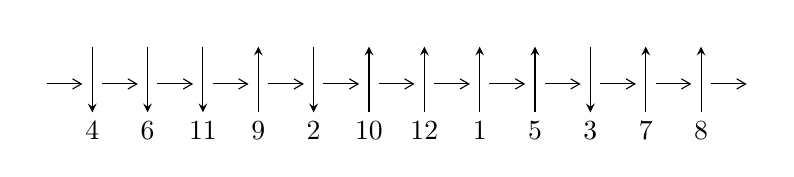
\begin{tikzpicture}[x=20pt, y=17pt]
	% nodes
	\node (C0) at (0, 0) {};
	\node (C1) at (1, 0) {};
	\node (C1U) at (1, +1) {};
	\node (C1D) at (1, -1) {4};

	\node (C2) at (2, 0) {};
	\node (C2U) at (2, +1) {};
	\node (C2D) at (2, -1) {6};

	\node (C3) at (3, 0) {};
	\node (C3U) at (3, +1) {};
	\node (C3D) at (3, -1) {11};

	\node (C4) at (4, 0) {};
	\node (C4U) at (4, +1) {};
	\node (C4D) at (4, -1) {9};

	\node (C5) at (5, 0) {};
	\node (C5U) at (5, +1) {};
	\node (C5D) at (5, -1) {2};

	\node (C6) at (6, 0) {};
	\node (C6U) at (6, +1) {};
	\node (C6D) at (6, -1) {10};

	\node (C7) at (7, 0) {};
	\node (C7U) at (7, +1) {};
	\node (C7D) at (7, -1) {12};

	\node (C8) at (8, 0) {};
	\node (C8U) at (8, +1) {};
	\node (C8D) at (8, -1) {1};

	\node (C9) at (9, 0) {};
	\node (C9U) at (9, +1) {};
	\node (C9D) at (9, -1) {5};

	\node (C10) at (10, 0) {};
	\node (C10U) at (10, +1) {};
	\node (C10D) at (10, -1) {3};

	\node (C11) at (11, 0) {};
	\node (C11U) at (11, +1) {};
	\node (C11D) at (11, -1) {7};

	\node (C12) at (12, 0) {};
	\node (C12U) at (12, +1) {};
	\node (C12D) at (12, -1) {8};
	\node (C13) at (13, 0) {};

	% arrows
	\draw[->,>={angle 60}]
	(C0) edge (C1) (C1) edge (C2) (C2) edge (C3) (C3) edge (C4) (C4) edge (C5) (C5) edge (C6) (C6) edge (C7) (C7) edge (C8) (C8) edge (C9) (C9) edge (C10) (C10) edge (C11) (C11) edge (C12) (C12) edge (C13) ;	\draw[->,>=stealth]
	(C1U) edge (C1D) (C2U) edge (C2D) (C3U) edge (C3D) (C4D) edge (C4U) (C5U) edge (C5D) (C6D) edge (C6U) (C7D) edge (C7U) (C8D) edge (C8U) (C9D) edge (C9U) (C10U) edge (C10D) (C11D) edge (C11U) (C12D) edge (C12U) ;
	\end{tikzpicture} \\
\hhline{~~} \\& 
\textbf{Solving Sequence} \\ \cline{2-2} 
 &
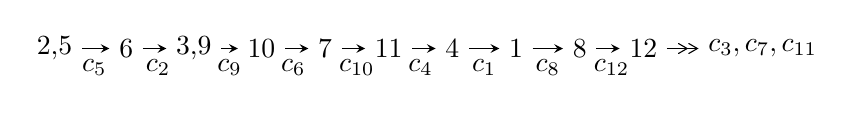
\begin{tikzpicture}[x=23pt, y=7pt]
	% node
	\node (A0) at (-1/8, 0) {2,5};
	\node (A1) at (1, 0) {6};
	\node (A2) at (33/16, 0) {3,9};
	\node (A3) at (25/8, 0) {10};
	\node (A4) at (33/8, 0) {7};
	\node (A5) at (41/8, 0) {11};
	\node (A6) at (49/8, 0) {4};
	\node (A7) at (57/8, 0) {1};
	\node (A8) at (65/8, 0) {8};
	\node (A9) at (73/8, 0) {12};
	\node (C1) at (1/2, -1) {$c_{5}$};
	\node (C2) at (3/2, -1) {$c_{2}$};
	\node (C3) at (21/8, -1) {$c_{9}$};
	\node (C4) at (29/8, -1) {$c_{6}$};
	\node (C5) at (37/8, -1) {$c_{10}$};
	\node (C6) at (45/8, -1) {$c_{4}$};
	\node (C7) at (53/8, -1) {$c_{1}$};
	\node (C8) at (61/8, -1) {$c_{8}$};
	\node (C9) at (69/8, -1) {$c_{12}$};
	\node (A10) at (11, 0) {$c_{3},c_{7},c_{11}$};

	% edge
	\draw[->,>=stealth]	
	(A0) edge (A1) (A1) edge (A2) (A2) edge (A3) (A3) edge (A4) (A4) edge (A5) (A5) edge (A6) (A6) edge (A7) (A7) edge (A8) (A8) edge (A9) ;
	\draw[->>,>={angle 60}]	
	(A9) edge (A10);
\end{tikzpicture} \\ 

\end{tabular} \\

\footnotetext{
The image of knot diagram is generated by the software ``\textbf{Draw programme}" developed by Andrew Bartholomew(\url{http://www.layer8.co.uk/maths/draw/index.htm\#Running-draw}), where we modified some parts for our purpose(\url{https://github.com/CATsTAILs/LinksPainter}).
}\phantom \\ \newline 
\centering \textbf{Ideals for irreducible components\footnotemark of $X_{\text{par}}$} 
 
\begin{align*}
I^u_{1}&=\langle 
-1747 u^{50}+78946 u^{49}+\cdots+1990656 b-43767094,\\
\phantom{I^u_{1}}&\phantom{= \langle  }-14055938 u^{50}+67741913 u^{49}+\cdots+279355392 a-5726762096,\\
\phantom{I^u_{1}}&\phantom{= \langle  }u^{51}-6 u^{50}+\cdots+8662 u-842\rangle \\
I^u_{2}&=\langle 
- a^2+b- a,\;a^3+2 a^2+a+1,\;u+1\rangle \\
I^u_{3}&=\langle 
b^4 a^2+2 b^3 a-2 b^2 a^2- b^2 a+b^2-2 b a+a^2- b+a-1,\;u+1\rangle \\
\\
I^v_{1}&=\langle 
a,\;b^6-2 b^4- b^3+b^2+b-1,\;v-1\rangle \\
I^v_{2}&=\langle 
a,\;b+1,\;v-1\rangle \\
\end{align*}
\raggedright * 4 irreducible components of $\dim_{\mathbb{C}}=0$, with total 61 representations.\\
\raggedright * 1 irreducible components of $\dim_{\mathbb{C}}=1$ \\
\footnotetext{All coefficients of polynomials are rational numbers. But the coefficients are sometimes approximated in decimal forms when there is not enough margin.}
\newpage
\renewcommand{\arraystretch}{1}
\centering \section*{I. $I^u_{1}= \langle -1747 u^{50}+7.89\times10^{4} u^{49}+\cdots+1.99\times10^{6} b-4.38\times10^{7},\;-1.41\times10^{7} u^{50}+6.77\times10^{7} u^{49}+\cdots+2.79\times10^{8} a-5.73\times10^{9},\;u^{51}-6 u^{50}+\cdots+8662 u-842 \rangle$}
\flushleft \textbf{(i) Arc colorings}\\
\begin{tabular}{m{7pt} m{180pt} m{7pt} m{180pt} }
\flushright $a_{2}=$&$\begin{pmatrix}0\\u\end{pmatrix}$ \\
\flushright $a_{5}=$&$\begin{pmatrix}1\\0\end{pmatrix}$ \\
\flushright $a_{6}=$&$\begin{pmatrix}1\\u^2\end{pmatrix}$ \\
\flushright $a_{3}=$&$\begin{pmatrix}- u\\- u^3+u\end{pmatrix}$ \\
\flushright $a_{9}=$&$\begin{pmatrix}0.0503156 u^{50}-0.242494 u^{49}+\cdots-256.094 u+20.4999\\0.000877600 u^{50}-0.0396583 u^{49}+\cdots-185.410 u+21.9863\end{pmatrix}$ \\
\flushright $a_{10}=$&$\begin{pmatrix}0.0511932 u^{50}-0.282152 u^{49}+\cdots-441.504 u+42.4862\\0.000877600 u^{50}-0.0396583 u^{49}+\cdots-185.410 u+21.9863\end{pmatrix}$ \\
\flushright $a_{7}=$&$\begin{pmatrix}0.0185165 u^{50}-0.0729252 u^{49}+\cdots-12.3427 u+3.52550\\0.0182020 u^{50}-0.0910577 u^{49}+\cdots-146.302 u+15.3639\end{pmatrix}$ \\
\flushright $a_{11}=$&$\begin{pmatrix}-0.0685537 u^{50}+0.309278 u^{49}+\cdots+380.668 u-44.0036\\0.00243739 u^{50}-0.00644160 u^{49}+\cdots-7.88344 u+1.49815\end{pmatrix}$ \\
\flushright $a_{4}=$&$\begin{pmatrix}0.0211970 u^{50}-0.106355 u^{49}+\cdots-161.802 u+15.3309\\-0.00435384 u^{50}+0.0207994 u^{49}+\cdots+26.1973 u-2.31048\end{pmatrix}$ \\
\flushright $a_{1}=$&$\begin{pmatrix}-0.00426257 u^{50}+0.0286204 u^{49}+\cdots+70.7619 u-7.40462\\0.0330833 u^{50}-0.152421 u^{49}+\cdots-177.572 u+18.3423\end{pmatrix}$ \\
\flushright $a_{8}=$&$\begin{pmatrix}0.114056 u^{50}-0.513210 u^{49}+\cdots-473.287 u+40.8488\\0.0646460 u^{50}-0.330940 u^{49}+\cdots-491.932 u+52.8520\end{pmatrix}$ \\
\flushright $a_{12}=$&$\begin{pmatrix}0.0705646 u^{50}-0.342297 u^{49}+\cdots-486.734 u+50.5146\\0.0477518 u^{50}-0.225647 u^{49}+\cdots-248.299 u+25.3200\end{pmatrix}$\\&\end{tabular}
\flushleft \textbf{(ii) Obstruction class $= -1$}\\~\\
\flushleft \textbf{(iii) Cusp Shapes $= -\frac{383093}{1492992} u^{50}+\frac{3585271}{2985984} u^{49}+\cdots+\frac{86360671}{55296} u-\frac{228139061}{1492992}$}\\~\\
\newpage\renewcommand{\arraystretch}{1}
\flushleft \textbf{(iv) u-Polynomials at the component}\newline \\
\begin{tabular}{m{50pt}|m{274pt}}
Crossings & \hspace{64pt}u-Polynomials at each crossing \\
\hline $$\begin{aligned}c_{1}\end{aligned}$$&$\begin{aligned}
&16(16 u^{51}+84 u^{49}+\cdots-138159 u-46107)
\end{aligned}$\\
\hline $$\begin{aligned}c_{2},c_{5}\end{aligned}$$&$\begin{aligned}
&u^{51}-6 u^{50}+\cdots+8662 u-842
\end{aligned}$\\
\hline $$\begin{aligned}c_{3},c_{10}\end{aligned}$$&$\begin{aligned}
&9(9 u^{51}-18 u^{50}+\cdots+3 u-1)
\end{aligned}$\\
\hline $$\begin{aligned}c_{4},c_{9}\end{aligned}$$&$\begin{aligned}
&9(9 u^{51}+18 u^{50}+\cdots- u-1)
\end{aligned}$\\
\hline $$\begin{aligned}c_{6}\end{aligned}$$&$\begin{aligned}
&16(16 u^{51}-16 u^{50}+\cdots-333 u+261)
\end{aligned}$\\
\hline $$\begin{aligned}c_{7},c_{8},c_{11}\\c_{12}\end{aligned}$$&$\begin{aligned}
&u^{51}-4 u^{50}+\cdots-186 u-46
\end{aligned}$\\
\hline
\end{tabular}\\~\\
\newpage\renewcommand{\arraystretch}{1}
\flushleft \textbf{(v) Riley Polynomials at the component}\newline \\
\begin{tabular}{m{50pt}|m{274pt}}
Crossings & \hspace{64pt}Riley Polynomials at each crossing \\
\hline $$\begin{aligned}c_{1}\end{aligned}$$&$\begin{aligned}
&256(256 y^{51}+2688 y^{50}+\cdots-3.63961\times10^{9} y-2.12586\times10^{9})
\end{aligned}$\\
\hline $$\begin{aligned}c_{2},c_{5}\end{aligned}$$&$\begin{aligned}
&y^{51}-34 y^{50}+\cdots+30048920 y-708964
\end{aligned}$\\
\hline $$\begin{aligned}c_{3},c_{10}\end{aligned}$$&$\begin{aligned}
&81(81 y^{51}-2376 y^{50}+\cdots+27 y-1)
\end{aligned}$\\
\hline $$\begin{aligned}c_{4},c_{9}\end{aligned}$$&$\begin{aligned}
&81(81 y^{51}-3024 y^{50}+\cdots+11 y-1)
\end{aligned}$\\
\hline $$\begin{aligned}c_{6}\end{aligned}$$&$\begin{aligned}
&256(256 y^{51}-3200 y^{50}+\cdots-3345273 y-68121)
\end{aligned}$\\
\hline $$\begin{aligned}c_{7},c_{8},c_{11}\\c_{12}\end{aligned}$$&$\begin{aligned}
&y^{51}-60 y^{50}+\cdots+35976 y-2116
\end{aligned}$\\
\hline
\end{tabular}\\~\\
\newpage\flushleft \textbf{(vi) Complex Volumes and Cusp Shapes}
$$\begin{array}{c|c|c}  
\text{Solutions to }I^u_{1}& \I (\text{vol} + \sqrt{-1}CS) & \text{Cusp shape}\\
 \hline 
\begin{aligned}
u &= \phantom{-}0.871937 + 0.599275 I \\
a &= -1.43039 - 0.76680 I \\
b &= \phantom{-}1.075950 - 0.106403 I\end{aligned}
 & \phantom{-}1.61712 - 0.65965 I & \phantom{-}7.95896 - 0.68823 I \\ \hline\begin{aligned}
u &= \phantom{-}0.871937 - 0.599275 I \\
a &= -1.43039 + 0.76680 I \\
b &= \phantom{-}1.075950 + 0.106403 I\end{aligned}
 & \phantom{-}1.61712 + 0.65965 I & \phantom{-}7.95896 + 0.68823 I \\ \hline\begin{aligned}
u &= -0.954975 + 0.488693 I \\
a &= \phantom{-}1.183620 + 0.097225 I \\
b &= \phantom{-}0.055327 - 0.421750 I\end{aligned}
 & \phantom{-}4.92043 - 1.04343 I & \phantom{-}                -6
0.500387 + 0. 10   I\phantom{ +0.000000I} \\ \hline\begin{aligned}
u &= -0.954975 - 0.488693 I \\
a &= \phantom{-}1.183620 - 0.097225 I \\
b &= \phantom{-}0.055327 + 0.421750 I\end{aligned}
 & \phantom{-}4.92043 + 1.04343 I & \phantom{-}                -6
0.500387 + 0. 10   I\phantom{ +0.000000I} \\ \hline\begin{aligned}
u &= \phantom{-}0.288710 + 0.865056 I \\
a &= \phantom{-}1.49117 + 0.44766 I \\
b &= -1.271070 - 0.230386 I\end{aligned}
 & \phantom{-}6.15912 + 2.38142 I & \phantom{-}10.95071 - 1.99222 I \\ \hline\begin{aligned}
u &= \phantom{-}0.288710 - 0.865056 I \\
a &= \phantom{-}1.49117 - 0.44766 I \\
b &= -1.271070 + 0.230386 I\end{aligned}
 & \phantom{-}6.15912 - 2.38142 I & \phantom{-}10.95071 + 1.99222 I \\ \hline\begin{aligned}
u &= \phantom{-}0.190005 + 0.889876 I \\
a &= -1.57561 - 0.59687 I \\
b &= \phantom{-}1.44689 + 0.33886 I\end{aligned}
 & \phantom{-}15.4058 + 4.1385 I & \phantom{-}11.16132 - 1.35851 I \\ \hline\begin{aligned}
u &= \phantom{-}0.190005 - 0.889876 I \\
a &= -1.57561 + 0.59687 I \\
b &= \phantom{-}1.44689 - 0.33886 I\end{aligned}
 & \phantom{-}15.4058 - 4.1385 I & \phantom{-}11.16132 + 1.35851 I \\ \hline\begin{aligned}
u &= -0.864821\phantom{ +0.000000I} \\
a &= -0.975469\phantom{ +0.000000I} \\
b &= -0.447949\phantom{ +0.000000I}\end{aligned}
 & -1.39737\phantom{ +0.000000I} & -9.01210\phantom{ +0.000000I} \\ \hline\begin{aligned}
u &= \phantom{-}0.063386 + 1.145060 I \\
a &= -1.72917 + 0.07049 I \\
b &= \phantom{-}1.39200 - 0.36995 I\end{aligned}
 & \phantom{-}12.5583 - 9.7853 I & \phantom{-}8.08488 + 5.85275 I\\
 \hline 
 \end{array}$$\newpage$$\begin{array}{c|c|c}  
\text{Solutions to }I^u_{1}& \I (\text{vol} + \sqrt{-1}CS) & \text{Cusp shape}\\
 \hline 
\begin{aligned}
u &= \phantom{-}0.063386 - 1.145060 I \\
a &= -1.72917 - 0.07049 I \\
b &= \phantom{-}1.39200 + 0.36995 I\end{aligned}
 & \phantom{-}12.5583 + 9.7853 I & \phantom{-}8.08488 - 5.85275 I \\ \hline\begin{aligned}
u &= \phantom{-}1.071180 + 0.478231 I \\
a &= \phantom{-}1.11714 + 1.01410 I \\
b &= -1.126820 + 0.397205 I\end{aligned}
 & \phantom{-}0.37782 - 4.14573 I & \phantom{-0.000000 -}0. + 5.58002 I \\ \hline\begin{aligned}
u &= \phantom{-}1.071180 - 0.478231 I \\
a &= \phantom{-}1.11714 - 1.01410 I \\
b &= -1.126820 - 0.397205 I\end{aligned}
 & \phantom{-}0.37782 + 4.14573 I & \phantom{-0.000000 } 0. - 5.58002 I \\ \hline\begin{aligned}
u &= -1.20895\phantom{ +0.000000I} \\
a &= \phantom{-}0.563495\phantom{ +0.000000I} \\
b &= \phantom{-}0.856182\phantom{ +0.000000I}\end{aligned}
 & \phantom{-}0.370489\phantom{ +0.000000I} & \phantom{-}11.3980\phantom{ +0.000000I} \\ \hline\begin{aligned}
u &= \phantom{-}1.22486\phantom{ +0.000000I} \\
a &= \phantom{-}1.64302\phantom{ +0.000000I} \\
b &= \phantom{-}0.210756\phantom{ +0.000000I}\end{aligned}
 & \phantom{-}6.17402\phantom{ +0.000000I} & -3.35810\phantom{ +0.000000I} \\ \hline\begin{aligned}
u &= -0.133856 + 0.749902 I \\
a &= -0.218006 + 0.669940 I \\
b &= -0.279882 - 0.872377 I\end{aligned}
 & \phantom{-}7.32400 + 5.35250 I & \phantom{-}5.78289 - 4.81378 I \\ \hline\begin{aligned}
u &= -0.133856 - 0.749902 I \\
a &= -0.218006 - 0.669940 I \\
b &= -0.279882 + 0.872377 I\end{aligned}
 & \phantom{-}7.32400 - 5.35250 I & \phantom{-}5.78289 + 4.81378 I \\ \hline\begin{aligned}
u &= \phantom{-}1.151360 + 0.486900 I \\
a &= -1.031110 - 0.933045 I \\
b &= \phantom{-}1.33347 - 0.56033 I\end{aligned}
 & \phantom{-}3.45393 - 7.28871 I & \phantom{-0.000000 } 0 \\ \hline\begin{aligned}
u &= \phantom{-}1.151360 - 0.486900 I \\
a &= -1.031110 + 0.933045 I \\
b &= \phantom{-}1.33347 + 0.56033 I\end{aligned}
 & \phantom{-}3.45393 + 7.28871 I & \phantom{-0.000000 } 0 \\ \hline\begin{aligned}
u &= \phantom{-}0.116607 + 1.248630 I \\
a &= \phantom{-}1.55658 - 0.00466 I \\
b &= -1.258200 + 0.254835 I\end{aligned}
 & \phantom{-}3.85227 - 6.56215 I & \phantom{-0.000000 } 0\\
 \hline 
 \end{array}$$\newpage$$\begin{array}{c|c|c}  
\text{Solutions to }I^u_{1}& \I (\text{vol} + \sqrt{-1}CS) & \text{Cusp shape}\\
 \hline 
\begin{aligned}
u &= \phantom{-}0.116607 - 1.248630 I \\
a &= \phantom{-}1.55658 + 0.00466 I \\
b &= -1.258200 - 0.254835 I\end{aligned}
 & \phantom{-}3.85227 + 6.56215 I & \phantom{-0.000000 } 0 \\ \hline\begin{aligned}
u &= \phantom{-}0.721707\phantom{ +0.000000I} \\
a &= \phantom{-}3.42336\phantom{ +0.000000I} \\
b &= -0.761960\phantom{ +0.000000I}\end{aligned}
 & \phantom{-}8.07048\phantom{ +0.000000I} & \phantom{-}15.1420\phantom{ +0.000000I} \\ \hline\begin{aligned}
u &= \phantom{-}1.185540 + 0.490657 I \\
a &= \phantom{-}1.035740 + 0.915650 I \\
b &= -1.51238 + 0.64262 I\end{aligned}
 & \phantom{-}12.3415 - 9.1062 I & \phantom{-0.000000 } 0 \\ \hline\begin{aligned}
u &= \phantom{-}1.185540 - 0.490657 I \\
a &= \phantom{-}1.035740 - 0.915650 I \\
b &= -1.51238 - 0.64262 I\end{aligned}
 & \phantom{-}12.3415 + 9.1062 I & \phantom{-0.000000 } 0 \\ \hline\begin{aligned}
u &= -0.222036 + 0.676897 I \\
a &= \phantom{-}0.395217 - 0.289769 I \\
b &= \phantom{-}0.196870 + 0.589331 I\end{aligned}
 & -0.49730 + 3.53349 I & \phantom{-}2.22017 - 7.44112 I \\ \hline\begin{aligned}
u &= -0.222036 - 0.676897 I \\
a &= \phantom{-}0.395217 + 0.289769 I \\
b &= \phantom{-}0.196870 - 0.589331 I\end{aligned}
 & -0.49730 - 3.53349 I & \phantom{-}2.22017 + 7.44112 I \\ \hline\begin{aligned}
u &= -0.489136 + 0.507443 I \\
a &= -0.863036 - 0.069456 I \\
b &= -0.124638 - 0.153724 I\end{aligned}
 & -1.58698 + 0.44085 I & -4.04045 - 0.10164 I \\ \hline\begin{aligned}
u &= -0.489136 - 0.507443 I \\
a &= -0.863036 + 0.069456 I \\
b &= -0.124638 + 0.153724 I\end{aligned}
 & -1.58698 - 0.44085 I & -4.04045 + 0.10164 I \\ \hline\begin{aligned}
u &= \phantom{-}1.284590 + 0.367030 I \\
a &= -0.415487 - 0.264559 I \\
b &= \phantom{-}0.160260 - 1.287920 I\end{aligned}
 & \phantom{-}3.01762 - 9.37305 I & \phantom{-0.000000 } 0 \\ \hline\begin{aligned}
u &= \phantom{-}1.284590 - 0.367030 I \\
a &= -0.415487 + 0.264559 I \\
b &= \phantom{-}0.160260 + 1.287920 I\end{aligned}
 & \phantom{-}3.01762 + 9.37305 I & \phantom{-0.000000 } 0\\
 \hline 
 \end{array}$$\newpage$$\begin{array}{c|c|c}  
\text{Solutions to }I^u_{1}& \I (\text{vol} + \sqrt{-1}CS) & \text{Cusp shape}\\
 \hline 
\begin{aligned}
u &= \phantom{-}1.301300 + 0.341701 I \\
a &= \phantom{-}0.201290 + 0.276131 I \\
b &= -0.027671 + 1.082990 I\end{aligned}
 & -5.08700 - 7.24377 I & \phantom{-0.000000 } 0 \\ \hline\begin{aligned}
u &= \phantom{-}1.301300 - 0.341701 I \\
a &= \phantom{-}0.201290 - 0.276131 I \\
b &= -0.027671 - 1.082990 I\end{aligned}
 & -5.08700 + 7.24377 I & \phantom{-0.000000 } 0 \\ \hline\begin{aligned}
u &= \phantom{-}1.337140 + 0.307386 I \\
a &= \phantom{-}0.068553 - 0.241472 I \\
b &= -0.132614 - 0.848734 I\end{aligned}
 & -6.92934 - 3.57492 I & \phantom{-0.000000 } 0 \\ \hline\begin{aligned}
u &= \phantom{-}1.337140 - 0.307386 I \\
a &= \phantom{-}0.068553 + 0.241472 I \\
b &= -0.132614 + 0.848734 I\end{aligned}
 & -6.92934 + 3.57492 I & \phantom{-0.000000 } 0 \\ \hline\begin{aligned}
u &= \phantom{-}1.40404 + 0.19556 I \\
a &= -0.500238 + 0.206535 I \\
b &= \phantom{-}0.226409 + 0.417307 I\end{aligned}
 & -3.34999 - 0.41537 I & \phantom{-0.000000 } 0 \\ \hline\begin{aligned}
u &= \phantom{-}1.40404 - 0.19556 I \\
a &= -0.500238 - 0.206535 I \\
b &= \phantom{-}0.226409 - 0.417307 I\end{aligned}
 & -3.34999 + 0.41537 I & \phantom{-0.000000 } 0 \\ \hline\begin{aligned}
u &= \phantom{-}0.52748 + 1.35639 I \\
a &= -1.345560 - 0.200993 I \\
b &= \phantom{-}1.163450 - 0.055837 I\end{aligned}
 & \phantom{-}1.80797 - 1.23291 I & \phantom{-0.000000 } 0 \\ \hline\begin{aligned}
u &= \phantom{-}0.52748 - 1.35639 I \\
a &= -1.345560 + 0.200993 I \\
b &= \phantom{-}1.163450 + 0.055837 I\end{aligned}
 & \phantom{-}1.80797 + 1.23291 I & \phantom{-0.000000 } 0 \\ \hline\begin{aligned}
u &= -1.38742 + 0.54293 I \\
a &= \phantom{-}1.15060 - 0.96574 I \\
b &= -1.44935 - 0.55020 I\end{aligned}
 & \phantom{-}8.0411 + 15.7082 I & \phantom{-0.000000 } 0 \\ \hline\begin{aligned}
u &= -1.38742 - 0.54293 I \\
a &= \phantom{-}1.15060 + 0.96574 I \\
b &= -1.44935 + 0.55020 I\end{aligned}
 & \phantom{-}8.0411 - 15.7082 I & \phantom{-0.000000 } 0\\
 \hline 
 \end{array}$$\newpage$$\begin{array}{c|c|c}  
\text{Solutions to }I^u_{1}& \I (\text{vol} + \sqrt{-1}CS) & \text{Cusp shape}\\
 \hline 
\begin{aligned}
u &= -1.40409 + 0.56693 I \\
a &= -1.121190 + 0.837048 I \\
b &= \phantom{-}1.34279 + 0.51016 I\end{aligned}
 & -0.81260 + 12.82570 I & \phantom{-0.000000 } 0 \\ \hline\begin{aligned}
u &= -1.40409 - 0.56693 I \\
a &= -1.121190 - 0.837048 I \\
b &= \phantom{-}1.34279 - 0.51016 I\end{aligned}
 & -0.81260 - 12.82570 I & \phantom{-0.000000 } 0 \\ \hline\begin{aligned}
u &= -1.54951 + 0.14699 I \\
a &= \phantom{-}0.172341 - 0.256428 I \\
b &= -1.170700 + 0.028166 I\end{aligned}
 & \phantom{-}9.83449 - 0.04248 I & \phantom{-0.000000 } 0 \\ \hline\begin{aligned}
u &= -1.54951 - 0.14699 I \\
a &= \phantom{-}0.172341 + 0.256428 I \\
b &= -1.170700 - 0.028166 I\end{aligned}
 & \phantom{-}9.83449 + 0.04248 I & \phantom{-0.000000 } 0 \\ \hline\begin{aligned}
u &= -1.43969 + 0.61276 I \\
a &= \phantom{-}1.067200 - 0.671303 I \\
b &= -1.214210 - 0.430814 I\end{aligned}
 & -3.57762 + 8.19895 I & \phantom{-0.000000 } 0 \\ \hline\begin{aligned}
u &= -1.43969 - 0.61276 I \\
a &= \phantom{-}1.067200 + 0.671303 I \\
b &= -1.214210 + 0.430814 I\end{aligned}
 & -3.57762 - 8.19895 I & \phantom{-0.000000 } 0 \\ \hline\begin{aligned}
u &= \phantom{-}1.37780 + 0.82539 I \\
a &= \phantom{-}0.906207 + 0.483019 I \\
b &= -1.213230 - 0.143156 I\end{aligned}
 & \phantom{-}8.68259 + 3.09879 I & \phantom{-0.000000 } 0 \\ \hline\begin{aligned}
u &= \phantom{-}1.37780 - 0.82539 I \\
a &= \phantom{-}0.906207 - 0.483019 I \\
b &= -1.213230 + 0.143156 I\end{aligned}
 & \phantom{-}8.68259 - 3.09879 I & \phantom{-0.000000 } 0 \\ \hline\begin{aligned}
u &= -1.60562 + 0.66191 I \\
a &= -0.900138 + 0.467041 I \\
b &= \phantom{-}1.127080 + 0.236987 I\end{aligned}
 & -0.72424 + 3.17343 I & \phantom{-0.000000 } 0 \\ \hline\begin{aligned}
u &= -1.60562 - 0.66191 I \\
a &= -0.900138 - 0.467041 I \\
b &= \phantom{-}1.127080 - 0.236987 I\end{aligned}
 & -0.72424 - 3.17343 I & \phantom{-0.000000 } 0\\
 \hline 
 \end{array}$$\newpage$$\begin{array}{c|c|c}  
\text{Solutions to }I^u_{1}& \I (\text{vol} + \sqrt{-1}CS) & \text{Cusp shape}\\
 \hline 
\begin{aligned}
u &= \phantom{-}0.157699\phantom{ +0.000000I} \\
a &= -4.50862\phantom{ +0.000000I} \\
b &= \phantom{-}0.663524\phantom{ +0.000000I}\end{aligned}
 & \phantom{-}0.907699\phantom{ +0.000000I} & \phantom{-}11.5760\phantom{ +0.000000I}\\
 \hline 
 \end{array}$$\newpage\newpage\renewcommand{\arraystretch}{1}
\centering \section*{II. $I^u_{2}= \langle - a^2+b- a,\;a^3+2 a^2+a+1,\;u+1 \rangle$}
\flushleft \textbf{(i) Arc colorings}\\
\begin{tabular}{m{7pt} m{180pt} m{7pt} m{180pt} }
\flushright $a_{2}=$&$\begin{pmatrix}0\\-1\end{pmatrix}$ \\
\flushright $a_{5}=$&$\begin{pmatrix}1\\0\end{pmatrix}$ \\
\flushright $a_{6}=$&$\begin{pmatrix}1\\1\end{pmatrix}$ \\
\flushright $a_{3}=$&$\begin{pmatrix}1\\0\end{pmatrix}$ \\
\flushright $a_{9}=$&$\begin{pmatrix}a\\a^2+a\end{pmatrix}$ \\
\flushright $a_{10}=$&$\begin{pmatrix}a^2+2 a\\a^2+a\end{pmatrix}$ \\
\flushright $a_{7}=$&$\begin{pmatrix}- a\\- a^2- a\end{pmatrix}$ \\
\flushright $a_{11}=$&$\begin{pmatrix}a\\a^2+a\end{pmatrix}$ \\
\flushright $a_{4}=$&$\begin{pmatrix}- a^2- a\\- a\end{pmatrix}$ \\
\flushright $a_{1}=$&$\begin{pmatrix}a\\a^2+a\end{pmatrix}$ \\
\flushright $a_{8}=$&$\begin{pmatrix}a\\a^2+a\end{pmatrix}$ \\
\flushright $a_{12}=$&$\begin{pmatrix}a\\a^2+a\end{pmatrix}$\\&\end{tabular}
\flushleft \textbf{(ii) Obstruction class $= -1$}\\~\\
\flushleft \textbf{(iii) Cusp Shapes $= -6$}\\~\\
\newpage\renewcommand{\arraystretch}{1}
\flushleft \textbf{(iv) u-Polynomials at the component}\newline \\
\begin{tabular}{m{50pt}|m{274pt}}
Crossings & \hspace{64pt}u-Polynomials at each crossing \\
\hline $$\begin{aligned}c_{1},c_{3},c_{4}\\c_{9},c_{10}\end{aligned}$$&$\begin{aligned}
&u^3- u-1
\end{aligned}$\\
\hline $$\begin{aligned}c_{2},c_{5}\end{aligned}$$&$\begin{aligned}
&(u+1)^3
\end{aligned}$\\
\hline $$\begin{aligned}c_{6}\end{aligned}$$&$\begin{aligned}
&u^3-2 u^2+u-1
\end{aligned}$\\
\hline $$\begin{aligned}c_{7},c_{8},c_{11}\\c_{12}\end{aligned}$$&$\begin{aligned}
&u^3
\end{aligned}$\\
\hline
\end{tabular}\\~\\
\newpage\renewcommand{\arraystretch}{1}
\flushleft \textbf{(v) Riley Polynomials at the component}\newline \\
\begin{tabular}{m{50pt}|m{274pt}}
Crossings & \hspace{64pt}Riley Polynomials at each crossing \\
\hline $$\begin{aligned}c_{1},c_{3},c_{4}\\c_{9},c_{10}\end{aligned}$$&$\begin{aligned}
&y^3-2 y^2+y-1
\end{aligned}$\\
\hline $$\begin{aligned}c_{2},c_{5}\end{aligned}$$&$\begin{aligned}
&(y-1)^3
\end{aligned}$\\
\hline $$\begin{aligned}c_{6}\end{aligned}$$&$\begin{aligned}
&y^3-2 y^2-3 y-1
\end{aligned}$\\
\hline $$\begin{aligned}c_{7},c_{8},c_{11}\\c_{12}\end{aligned}$$&$\begin{aligned}
&y^3
\end{aligned}$\\
\hline
\end{tabular}\\~\\
\newpage\flushleft \textbf{(vi) Complex Volumes and Cusp Shapes}
$$\begin{array}{c|c|c}  
\text{Solutions to }I^u_{2}& \I (\text{vol} + \sqrt{-1}CS) & \text{Cusp shape}\\
 \hline 
\begin{aligned}
u &= -1.00000\phantom{ +0.000000I} \\
a &= -0.122561 + 0.744862 I \\
b &= -0.662359 + 0.562280 I\end{aligned}
 & -1.64493\phantom{ +0.000000I} & -6.00000\phantom{ +0.000000I} \\ \hline\begin{aligned}
u &= -1.00000\phantom{ +0.000000I} \\
a &= -0.122561 - 0.744862 I \\
b &= -0.662359 - 0.562280 I\end{aligned}
 & -1.64493\phantom{ +0.000000I} & -6.00000\phantom{ +0.000000I} \\ \hline\begin{aligned}
u &= -1.00000\phantom{ +0.000000I} \\
a &= -1.75488\phantom{ +0.000000I} \\
b &= \phantom{-}1.32472\phantom{ +0.000000I}\end{aligned}
 & -1.64493\phantom{ +0.000000I} & -6.00000\phantom{ +0.000000I}\\
 \hline 
 \end{array}$$\newpage\newpage\renewcommand{\arraystretch}{1}
\centering \section*{III. $I^u_{3}= \langle b^4 a^2+2 b^3 a-2 b^2 a^2- b^2 a+b^2-2 b a+a^2- b+a-1,\;u+1 \rangle$}
\flushleft \textbf{(i) Arc colorings}\\
\begin{tabular}{m{7pt} m{180pt} m{7pt} m{180pt} }
\flushright $a_{2}=$&$\begin{pmatrix}0\\-1\end{pmatrix}$ \\
\flushright $a_{5}=$&$\begin{pmatrix}1\\0\end{pmatrix}$ \\
\flushright $a_{6}=$&$\begin{pmatrix}1\\1\end{pmatrix}$ \\
\flushright $a_{3}=$&$\begin{pmatrix}1\\0\end{pmatrix}$ \\
\flushright $a_{9}=$&$\begin{pmatrix}a\\b\end{pmatrix}$ \\
\flushright $a_{10}=$&$\begin{pmatrix}b+a\\b\end{pmatrix}$ \\
\flushright $a_{7}=$&$\begin{pmatrix}b a+a^2+1\\b a+1\end{pmatrix}$ \\
\flushright $a_{11}=$&$\begin{pmatrix}a\\b\end{pmatrix}$ \\
\flushright $a_{4}=$&$\begin{pmatrix}b a+1\\b^2\end{pmatrix}$ \\
\flushright $a_{1}=$&$\begin{pmatrix}- b^2 a^2-2 b a-1\\- b^3 a- b^2-1\end{pmatrix}$ \\
\flushright $a_{8}=$&$\begin{pmatrix}- b^3 a^2- a^3 b^2- b^2 a^2-2 b^2 a+a^3- b a+a^2- b+a\\- b^3 a^2- b^3 a-2 b^2 a+a^2 b- b^2+b a- b+a\end{pmatrix}$ \\
\flushright $a_{12}=$&$\begin{pmatrix}b^3 a^2+a^3 b^2+2 b^2 a- a^3+b\\b^3 a^2+2 b^2 a- a^2 b+2 b- a\end{pmatrix}$\\&\end{tabular}
\flushleft \textbf{(ii) Obstruction class $= 1$}\\~\\
\flushleft \textbf{(iii) Cusp Shapes $= 4$}\\~\\
\flushleft \textbf{(iv) u-Polynomials at the component} : It cannot be defined for a positive dimension component.\\~\\
\flushleft \textbf{(v) Riley Polynomials at the component} : It cannot be defined for a positive dimension component.\\~\\
\newpage\flushleft \textbf{(iv) Complex Volumes and Cusp Shapes}
$$\begin{array}{c|c|c} 
\text{Solution to }I^u_{3}& \I (\text{vol} + \sqrt{-1}CS) & \text{Cusp shape}\\
 \hline 
\begin{aligned}
u &= \cdots \\
a &= \cdots \\
b &= \cdots\end{aligned}
 & \phantom{-}7.23771\phantom{ +0.000000I} & \phantom{-}4.00000\phantom{ +0.000000I}\\
 \hline 
 \end{array}
$$\newpage\renewcommand{\arraystretch}{1}
\centering \section*{IV. $I^v_{1}= \langle a,\;b^6-2 b^4- b^3+b^2+b-1,\;v-1 \rangle$}
\flushleft \textbf{(i) Arc colorings}\\
\begin{tabular}{m{7pt} m{180pt} m{7pt} m{180pt} }
\flushright $a_{2}=$&$\begin{pmatrix}1\\0\end{pmatrix}$ \\
\flushright $a_{5}=$&$\begin{pmatrix}1\\0\end{pmatrix}$ \\
\flushright $a_{6}=$&$\begin{pmatrix}1\\0\end{pmatrix}$ \\
\flushright $a_{3}=$&$\begin{pmatrix}1\\0\end{pmatrix}$ \\
\flushright $a_{9}=$&$\begin{pmatrix}0\\b\end{pmatrix}$ \\
\flushright $a_{10}=$&$\begin{pmatrix}b\\b\end{pmatrix}$ \\
\flushright $a_{7}=$&$\begin{pmatrix}- b^2+1\\- b^2\end{pmatrix}$ \\
\flushright $a_{11}=$&$\begin{pmatrix}0\\b\end{pmatrix}$ \\
\flushright $a_{4}=$&$\begin{pmatrix}1\\b^2\end{pmatrix}$ \\
\flushright $a_{1}=$&$\begin{pmatrix}- b^2+1\\- b^4\end{pmatrix}$ \\
\flushright $a_{8}=$&$\begin{pmatrix}- b^5+2 b^3- b\\- b^5- b^4+b^3+b^2\end{pmatrix}$ \\
\flushright $a_{12}=$&$\begin{pmatrix}b^5-2 b^3+b\\b^5- b^3+b\end{pmatrix}$\\&\end{tabular}
\flushleft \textbf{(ii) Obstruction class $= -1$}\\~\\
\flushleft \textbf{(iii) Cusp Shapes $= 10$}\\~\\
\newpage\renewcommand{\arraystretch}{1}
\flushleft \textbf{(iv) u-Polynomials at the component}\newline \\
\begin{tabular}{m{50pt}|m{274pt}}
Crossings & \hspace{64pt}u-Polynomials at each crossing \\
\hline $$\begin{aligned}c_{1}\end{aligned}$$&$\begin{aligned}
&u^6+4 u^5+6 u^4+7 u^3+7 u^2+3 u+1
\end{aligned}$\\
\hline $$\begin{aligned}c_{2},c_{5}\end{aligned}$$&$\begin{aligned}
&u^6
\end{aligned}$\\
\hline $$\begin{aligned}c_{3},c_{4},c_{6}\\c_{9},c_{10}\end{aligned}$$&$\begin{aligned}
&u^6-2 u^4- u^3+u^2+u-1
\end{aligned}$\\
\hline $$\begin{aligned}c_{7},c_{8},c_{11}\\c_{12}\end{aligned}$$&$\begin{aligned}
&(u^2+u-1)^3
\end{aligned}$\\
\hline
\end{tabular}\\~\\
\newpage\renewcommand{\arraystretch}{1}
\flushleft \textbf{(v) Riley Polynomials at the component}\newline \\
\begin{tabular}{m{50pt}|m{274pt}}
Crossings & \hspace{64pt}Riley Polynomials at each crossing \\
\hline $$\begin{aligned}c_{1}\end{aligned}$$&$\begin{aligned}
&y^6-4 y^5-6 y^4+13 y^3+19 y^2+5 y+1
\end{aligned}$\\
\hline $$\begin{aligned}c_{2},c_{5}\end{aligned}$$&$\begin{aligned}
&y^6
\end{aligned}$\\
\hline $$\begin{aligned}c_{3},c_{4},c_{6}\\c_{9},c_{10}\end{aligned}$$&$\begin{aligned}
&y^6-4 y^5+6 y^4-7 y^3+7 y^2-3 y+1
\end{aligned}$\\
\hline $$\begin{aligned}c_{7},c_{8},c_{11}\\c_{12}\end{aligned}$$&$\begin{aligned}
&(y^2-3 y+1)^3
\end{aligned}$\\
\hline
\end{tabular}\\~\\
\newpage\flushleft \textbf{(vi) Complex Volumes and Cusp Shapes}
$$\begin{array}{c|c|c}  
\text{Solutions to }I^v_{1}& \I (\text{vol} + \sqrt{-1}CS) & \text{Cusp shape}\\
 \hline 
\begin{aligned}
v &= \phantom{-}1.00000\phantom{ +0.000000I} \\
a &= \phantom{-0.000000 } 0 \\
b &= -0.726823 + 0.764732 I\end{aligned}
 & \phantom{-}8.88264\phantom{ +0.000000I} & \phantom{-}10.0000\phantom{ +0.000000I} \\ \hline\begin{aligned}
v &= \phantom{-}1.00000\phantom{ +0.000000I} \\
a &= \phantom{-0.000000 } 0 \\
b &= -0.726823 - 0.764732 I\end{aligned}
 & \phantom{-}8.88264\phantom{ +0.000000I} & \phantom{-}10.0000\phantom{ +0.000000I} \\ \hline\begin{aligned}
v &= \phantom{-}1.00000\phantom{ +0.000000I} \\
a &= \phantom{-0.000000 } 0 \\
b &= -1.22636\phantom{ +0.000000I}\end{aligned}
 & \phantom{-}0.986960\phantom{ +0.000000I} & \phantom{-}10.0000\phantom{ +0.000000I} \\ \hline\begin{aligned}
v &= \phantom{-}1.00000\phantom{ +0.000000I} \\
a &= \phantom{-0.000000 } 0 \\
b &= \phantom{-}0.613180 + 0.357727 I\end{aligned}
 & \phantom{-}0.986960\phantom{ +0.000000I} & \phantom{-}10.0000\phantom{ +0.000000I} \\ \hline\begin{aligned}
v &= \phantom{-}1.00000\phantom{ +0.000000I} \\
a &= \phantom{-0.000000 } 0 \\
b &= \phantom{-}0.613180 - 0.357727 I\end{aligned}
 & \phantom{-}0.986960\phantom{ +0.000000I} & \phantom{-}10.0000\phantom{ +0.000000I} \\ \hline\begin{aligned}
v &= \phantom{-}1.00000\phantom{ +0.000000I} \\
a &= \phantom{-0.000000 } 0 \\
b &= \phantom{-}1.45365\phantom{ +0.000000I}\end{aligned}
 & \phantom{-}8.88264\phantom{ +0.000000I} & \phantom{-}10.0000\phantom{ +0.000000I}\\
 \hline 
 \end{array}$$\newpage\newpage\renewcommand{\arraystretch}{1}
\centering \section*{V. $I^v_{2}= \langle a,\;b+1,\;v-1 \rangle$}
\flushleft \textbf{(i) Arc colorings}\\
\begin{tabular}{m{7pt} m{180pt} m{7pt} m{180pt} }
\flushright $a_{2}=$&$\begin{pmatrix}1\\0\end{pmatrix}$ \\
\flushright $a_{5}=$&$\begin{pmatrix}1\\0\end{pmatrix}$ \\
\flushright $a_{6}=$&$\begin{pmatrix}1\\0\end{pmatrix}$ \\
\flushright $a_{3}=$&$\begin{pmatrix}1\\0\end{pmatrix}$ \\
\flushright $a_{9}=$&$\begin{pmatrix}0\\-1\end{pmatrix}$ \\
\flushright $a_{10}=$&$\begin{pmatrix}-1\\-1\end{pmatrix}$ \\
\flushright $a_{7}=$&$\begin{pmatrix}0\\-1\end{pmatrix}$ \\
\flushright $a_{11}=$&$\begin{pmatrix}0\\-1\end{pmatrix}$ \\
\flushright $a_{4}=$&$\begin{pmatrix}1\\1\end{pmatrix}$ \\
\flushright $a_{1}=$&$\begin{pmatrix}0\\-1\end{pmatrix}$ \\
\flushright $a_{8}=$&$\begin{pmatrix}0\\-1\end{pmatrix}$ \\
\flushright $a_{12}=$&$\begin{pmatrix}0\\-1\end{pmatrix}$\\&\end{tabular}
\flushleft \textbf{(ii) Obstruction class $= 1$}\\~\\
\flushleft \textbf{(iii) Cusp Shapes $= 0$}\\~\\
\newpage\renewcommand{\arraystretch}{1}
\flushleft \textbf{(iv) u-Polynomials at the component}\newline \\
\begin{tabular}{m{50pt}|m{274pt}}
Crossings & \hspace{64pt}u-Polynomials at each crossing \\
\hline $$\begin{aligned}c_{1},c_{9},c_{10}\end{aligned}$$&$\begin{aligned}
&u-1
\end{aligned}$\\
\hline $$\begin{aligned}c_{2},c_{5},c_{7}\\c_{8},c_{11},c_{12}\end{aligned}$$&$\begin{aligned}
&u
\end{aligned}$\\
\hline $$\begin{aligned}c_{3},c_{4},c_{6}\end{aligned}$$&$\begin{aligned}
&u+1
\end{aligned}$\\
\hline
\end{tabular}\\~\\
\newpage\renewcommand{\arraystretch}{1}
\flushleft \textbf{(v) Riley Polynomials at the component}\newline \\
\begin{tabular}{m{50pt}|m{274pt}}
Crossings & \hspace{64pt}Riley Polynomials at each crossing \\
\hline $$\begin{aligned}c_{1},c_{3},c_{4}\\c_{6},c_{9},c_{10}\end{aligned}$$&$\begin{aligned}
&y-1
\end{aligned}$\\
\hline $$\begin{aligned}c_{2},c_{5},c_{7}\\c_{8},c_{11},c_{12}\end{aligned}$$&$\begin{aligned}
&y
\end{aligned}$\\
\hline
\end{tabular}\\~\\
\newpage\flushleft \textbf{(vi) Complex Volumes and Cusp Shapes}
$$\begin{array}{c|c|c}  
\text{Solutions to }I^v_{2}& \I (\text{vol} + \sqrt{-1}CS) & \text{Cusp shape}\\
 \hline 
\begin{aligned}
v &= \phantom{-}1.00000\phantom{ +0.000000I} \\
a &= \phantom{-0.000000 } 0 \\
b &= -1.00000\phantom{ +0.000000I}\end{aligned}
 & \phantom{-0.000000 } 0 & \phantom{-0.000000 } 0\\
 \hline 
 \end{array}$$\newpage
\newpage\renewcommand{\arraystretch}{1}
\centering \section*{ VI. u-Polynomials}
\begin{tabular}{m{50pt}|m{274pt}}
Crossings & \hspace{64pt}u-Polynomials at each crossing \\
\hline $$\begin{aligned}c_{1}\end{aligned}$$&$\begin{aligned}
&16(u-1)(u^3- u-1)(u^6+4 u^5+6 u^4+7 u^3+7 u^2+3 u+1)\\
&\cdot(16 u^{51}+84 u^{49}+\cdots-138159 u-46107)
\end{aligned}$\\
\hline $$\begin{aligned}c_{2},c_{5}\end{aligned}$$&$\begin{aligned}
&u^7(u+1)^3(u^{51}-6 u^{50}+\cdots+8662 u-842)
\end{aligned}$\\
\hline $$\begin{aligned}c_{3}\end{aligned}$$&$\begin{aligned}
&9(u+1)(u^3- u-1)(u^6-2 u^4- u^3+u^2+u-1)\\
&\cdot(9 u^{51}-18 u^{50}+\cdots+3 u-1)
\end{aligned}$\\
\hline $$\begin{aligned}c_{4}\end{aligned}$$&$\begin{aligned}
&9(u+1)(u^3- u-1)(u^{6}-2 u^{4}+\cdots+u-1)(9 u^{51}+18 u^{50}+\cdots-u-1)
\end{aligned}$\\
\hline $$\begin{aligned}c_{6}\end{aligned}$$&$\begin{aligned}
&16(u+1)(u^3-2 u^2+u-1)(u^6-2 u^4- u^3+u^2+u-1)\\
&\cdot(16 u^{51}-16 u^{50}+\cdots-333 u+261)
\end{aligned}$\\
\hline $$\begin{aligned}c_{7},c_{8},c_{11}\\c_{12}\end{aligned}$$&$\begin{aligned}
&u^4(u^2+u-1)^3(u^{51}-4 u^{50}+\cdots-186 u-46)
\end{aligned}$\\
\hline $$\begin{aligned}c_{9}\end{aligned}$$&$\begin{aligned}
&9(u-1)(u^3- u-1)(u^{6}-2 u^{4}+\cdots+u-1)(9 u^{51}+18 u^{50}+\cdots-u-1)
\end{aligned}$\\
\hline $$\begin{aligned}c_{10}\end{aligned}$$&$\begin{aligned}
&9(u-1)(u^3- u-1)(u^6-2 u^4- u^3+u^2+u-1)\\
&\cdot(9 u^{51}-18 u^{50}+\cdots+3 u-1)
\end{aligned}$\\
\hline
\end{tabular}\newpage\renewcommand{\arraystretch}{1}
\centering \section*{ VII. Riley Polynomials}
\begin{tabular}{m{50pt}|m{274pt}}
Crossings & \hspace{64pt}Riley Polynomials at each crossing \\
\hline $$\begin{aligned}c_{1}\end{aligned}$$&$\begin{aligned}
&256(y-1)(y^3-2 y^2+y-1)(y^{6}-4 y^{5}+\cdots+5 y+1)\\
&\cdot(256 y^{51}+2688 y^{50}+\cdots-3639614229 y-2125855449)
\end{aligned}$\\
\hline $$\begin{aligned}c_{2},c_{5}\end{aligned}$$&$\begin{aligned}
&y^7(y-1)^3(y^{51}-34 y^{50}+\cdots+3.00489\times10^{7} y-708964)
\end{aligned}$\\
\hline $$\begin{aligned}c_{3},c_{10}\end{aligned}$$&$\begin{aligned}
&81(y-1)(y^3-2 y^2+y-1)(y^6-4 y^5+6 y^4-7 y^3+7 y^2-3 y+1)\\
&\cdot(81 y^{51}-2376 y^{50}+\cdots+27 y-1)
\end{aligned}$\\
\hline $$\begin{aligned}c_{4},c_{9}\end{aligned}$$&$\begin{aligned}
&81(y-1)(y^3-2 y^2+y-1)(y^6-4 y^5+6 y^4-7 y^3+7 y^2-3 y+1)\\
&\cdot(81 y^{51}-3024 y^{50}+\cdots+11 y-1)
\end{aligned}$\\
\hline $$\begin{aligned}c_{6}\end{aligned}$$&$\begin{aligned}
&256(y-1)(y^{3}-2 y^{2}-3 y-1)(y^{6}-4 y^{5}+\cdots-3 y+1)\\
&\cdot(256 y^{51}-3200 y^{50}+\cdots-3345273 y-68121)
\end{aligned}$\\
\hline $$\begin{aligned}c_{7},c_{8},c_{11}\\c_{12}\end{aligned}$$&$\begin{aligned}
&y^4(y^2-3 y+1)^3(y^{51}-60 y^{50}+\cdots+35976 y-2116)
\end{aligned}$\\
\hline
\end{tabular}
\vskip 2pc
\end{document}